\documentclass[aps,prb,onecolumn,notitlepage,showpacs,floatfix,superscriptaddress]{revtex4-1}
\usepackage{dcolumn}
\usepackage{tabularx}
\usepackage{bm}
\usepackage{soul}
\usepackage{amsmath,amssymb,graphicx}
\usepackage[colorlinks=true,citecolor=blue,urlcolor=blue,linkcolor=blue]{hyperref}
\usepackage{environ}

\NewEnviron{eqnsplit}{%
\begin{equation}
\begin{split}
  \BODY
\end{split}
\end{equation}
}

\newcommand{\mrm}[1]{\mathrm{#1}}
\newcommand{\ang}{\mathrm{\AA}}

\bibliographystyle{apsrev4-1}

%%%%%%%%%%%%%%%%%%%%%%%%%%%%%%%%%%%%%%%%%%%%%%%%
\begin{document}

\title{Spin Relaxation Mechanisms}

\author{Avinash Rustagi}
\email{arustag@ncsu.edu}
\affiliation{Department of Physics, North Carolina State University, Raleigh, NC 27695}
%
\date{\today}
%%%%%%%%%%%%%%%%%%%%%%%%%%%%%%%%%%%%%%%%%%%%%%%%
\begin{abstract}
Highlight the physics of some spin relaxation mechanisms
\end{abstract}

\maketitle
%
There are some common spin relaxation mechanisms:
\begin{itemize}
\item Elliot-Yafet
\item Dyakanov-Perel
\end{itemize}

\section{Symmetry}
\subsection{Time-Reversal Symmetry}
The time reversal symmetry implies that the system remains unchanged upon application of time-reversal operator. For an eigenstate characterized by quantum numbers $({\bm k},{\bm \sigma})$, time-reversal invariance means
\begin{equation}
\varepsilon_{{\bm k},{\bm \sigma}}=\varepsilon_{-{\bm k},-{\bm \sigma}}
\end{equation}
which means that for every state characterized by quantum numbers $({\bm k},{\bm \sigma})$, there is a degenerate state $(-{\bm k},-{\bm \sigma})$ also referred as \textbf{\textit{Kramers Degeneracy}}. The time-reversal operator $\hat{K}$ is expressed as
\begin{equation}
\hat{K}=-i\sigma_y \hat{C}
\end{equation}
where $\sigma_y$ is the y-Pauli matrix and $\hat{C}$ is the conjugation operator. Effects of $\hat{K}$:
\begin{equation}
\begin{split}
&{\bm k} \rightarrow -{\bm k} \\
&\vert \uparrow \rangle \rightarrow \vert \downarrow \rangle \\
&\vert \downarrow \rangle \rightarrow - \vert \uparrow \rangle \\
\end{split}
\end{equation}
Note: For a particle with spin $J$, the representation for the operator is 
\begin{equation}
\hat{K}=\exp\left( -i\pi J_y /\hbar\right) \hat{C}
\end{equation}
If spin 1/2: $J_y=\hbar \sigma_y/2$ which implies $\exp\left( -i\pi J_y /\hbar\right)=-i\sigma_y$. This uses the identity (for given unit vector ${\bm v}$)
\begin{equation}
\begin{split}
\exp\left( i \theta {\bm v}\cdot{\bm \sigma}\right) &= \sum_{k=0}^{\infty} \dfrac{1}{k\, !} \left( i \theta {\bm v}\cdot{\bm \sigma}\right)^k \\
&=\sum_{k=0}^{\infty} \dfrac{1}{(2k)\, !} \left( i \theta {\bm v}\cdot{\bm \sigma}\right)^{2k} +\sum_{k=0}^{\infty} \dfrac{1}{(2k+1)\, !} \left( i \theta {\bm v}\cdot{\bm \sigma}\right)^{2k+1} \\
&=\sum_{k=0}^{\infty} \dfrac{(-1)^k}{(2k)\, !} \theta^{2k} \left(  {\bm v}\cdot{\bm \sigma}\right)^{2k} +\sum_{k=0}^{\infty} \dfrac{i(-1)^k}{(2k+1)\, !} \theta^{2k+1} \left(  {\bm v}\cdot{\bm \sigma}\right)^{2k+1}
\end{split}
\end{equation}
Since $\left(  {\bm v}\cdot{\bm \sigma}\right)^{2k}=I$ given ${\bm v}$ is a unit vector. Therefore
\begin{equation}
\begin{split}
\exp\left( i \theta {\bm v}\cdot{\bm \sigma}\right) &=\sum_{k=0}^{\infty} \dfrac{(-1)^k}{(2k)\, !} \theta^{2k} I +\sum_{k=0}^{\infty} \dfrac{i(-1)^k}{(2k+1)\, !} \theta^{2k+1} \left(  {\bm v}\cdot{\bm \sigma}\right) \\
&= \cos(\theta)I + i \sin(\theta) {\bm v}\cdot{\bm \sigma}
\end{split}
\end{equation}
\subsection{Inversion Symmetry}
The spatial inversion symmetry implies that the system remains unchanged upon application of inversion operator $\hat{I}$. For an eigenstate characterized by quantum numbers $({\bm k},{\bm \sigma})$, time-reversal invariance means
\begin{equation}
\varepsilon_{{\bm k},{\bm \sigma}}=\varepsilon_{-{\bm k},{\bm \sigma}}
\end{equation}
which means that for every state characterized by quantum numbers $({\bm k},{\bm \sigma})$, there is a degenerate state $(-{\bm k},{\bm \sigma})$. Effects of $\hat{I}$:
\begin{equation}
\begin{split}
&{\bm k} \rightarrow -{\bm k} \\
&{\bm r} \rightarrow -{\bm r}
\end{split}
\end{equation}

\subsection{Time-Reversal and Inversion Symmetry}
When the system has both inversion and time-reversal symmetry
\begin{equation}
\varepsilon_{{\bm k},{\bm \sigma}}=\varepsilon_{-{\bm k},-{\bm \sigma}}=\varepsilon_{{\bm k},-{\bm \sigma}}=\varepsilon_{-{\bm k},{\bm \sigma}}
\end{equation}
which implies that for every state characterized by quantum numbers $({\bm k},{\bm \sigma})$, there is a degenerate state $({\bm k},-{\bm \sigma})$. 

\section{Elliot-Yafet Mechanism}
This mechanism is based on scattering in presence of spin-orbit coupling. We know that the presence of spin-orbit leads to mixing the the spin up/down eigenstates. Thus a general eigenfunction can be written as
\begin{equation}
\begin{split}
 \Psi_{{\bm k},n,+1/2} ({\bm r}) &= \left[a_{{\bm k},n}({\bm r}) \vert\uparrow \rangle +b_{{\bm k},n}({\bm r}) \vert\downarrow \rangle \right] e^{i{\bm k}\cdot{\bm r}} 
\end{split}
\end{equation}
Spin-Orbit Interaction preserves time-reversal symmetry, thus the time-reversed wavefunction has the same energy
\begin{equation}
\hat{K}\Psi_{{\bm k},n,+1/2} ({\bm r}) = \left[a^{*}_{-{\bm k},n}({\bm r}) \vert\downarrow \rangle - b^{*}_{-{\bm k},n}({\bm r}) \vert\uparrow \rangle \right] e^{i{\bm k}\cdot{\bm r}} \equiv \Psi_{-{\bm k},n,-1/2} ({\bm r})  
\end{equation}
Therefore
\begin{equation}
\Psi_{{\bm k},n,-1/2} ({\bm r})  = \left[a^{*}_{{\bm k},n}({\bm r}) \vert\downarrow \rangle - b^{*}_{{\bm k},n}({\bm r}) \vert\uparrow \rangle \right] e^{-i{\bm k}\cdot{\bm r}} 
\end{equation}
Now if a scattering event happens which does not act in spin space e.g. impurity or phonons, the momenta of the electron changes from ${\bm k} \rightarrow {\bm k}^\prime$. Thus the scattering probability to preserve/flip spin is
\begin{equation}
\begin{split}
P_{\vert\uparrow \rangle\rightarrow\vert\uparrow \rangle} &\propto \vert M_{{\bm k} ,{\bm k}^\prime} \vert^2 \vert a^*_{{\bm k}^\prime,n} a_{{\bm k},n}\vert^2 \\
P_{\vert\uparrow \rangle\rightarrow\vert\downarrow \rangle} &\propto \vert M_{{\bm k} ,{\bm k}^\prime} \vert^2 \vert b^*_{{\bm k}^\prime,n} a_{{\bm k},n}\vert^2
\end{split}
\end{equation}
This is the basic principle of Elliot-Yafet Spin Relaxation where non-spin-flip scattering events can lead to spin relaxation. \\
%
Physically, we expect scattering rate $\tau^{-1}$ increases with increase in temperature $T$. Thus we can conclude that with increase in temperature, the spin relaxation rate via Elliot-Yafet mechanism also increases.
\begin{equation}
\tau_{EY}^{-1} \propto \tau^{-1} \propto T
\end{equation}

\section{Dyakanov-Perel Mechanism}
If the system has both time-reversal and inversion symmetry
\begin{equation}
\varepsilon_{{\bm k},{\bm \sigma}}=\varepsilon_{-{\bm k},{\bm \sigma}}=\varepsilon_{{\bm k},-{\bm \sigma}}
\end{equation}
which implies that for a given ${\bm k}$, there are two degenerate wavefunctions corresponding to spin up and down. Now if the system lacks inversion (in semiconductor nanostructures), only time-reversal symmetry holds
\begin{equation}
\varepsilon_{{\bm k},{\bm \sigma}}=\varepsilon_{-{\bm k},-{\bm \sigma}}
\end{equation}
\begin{figure}
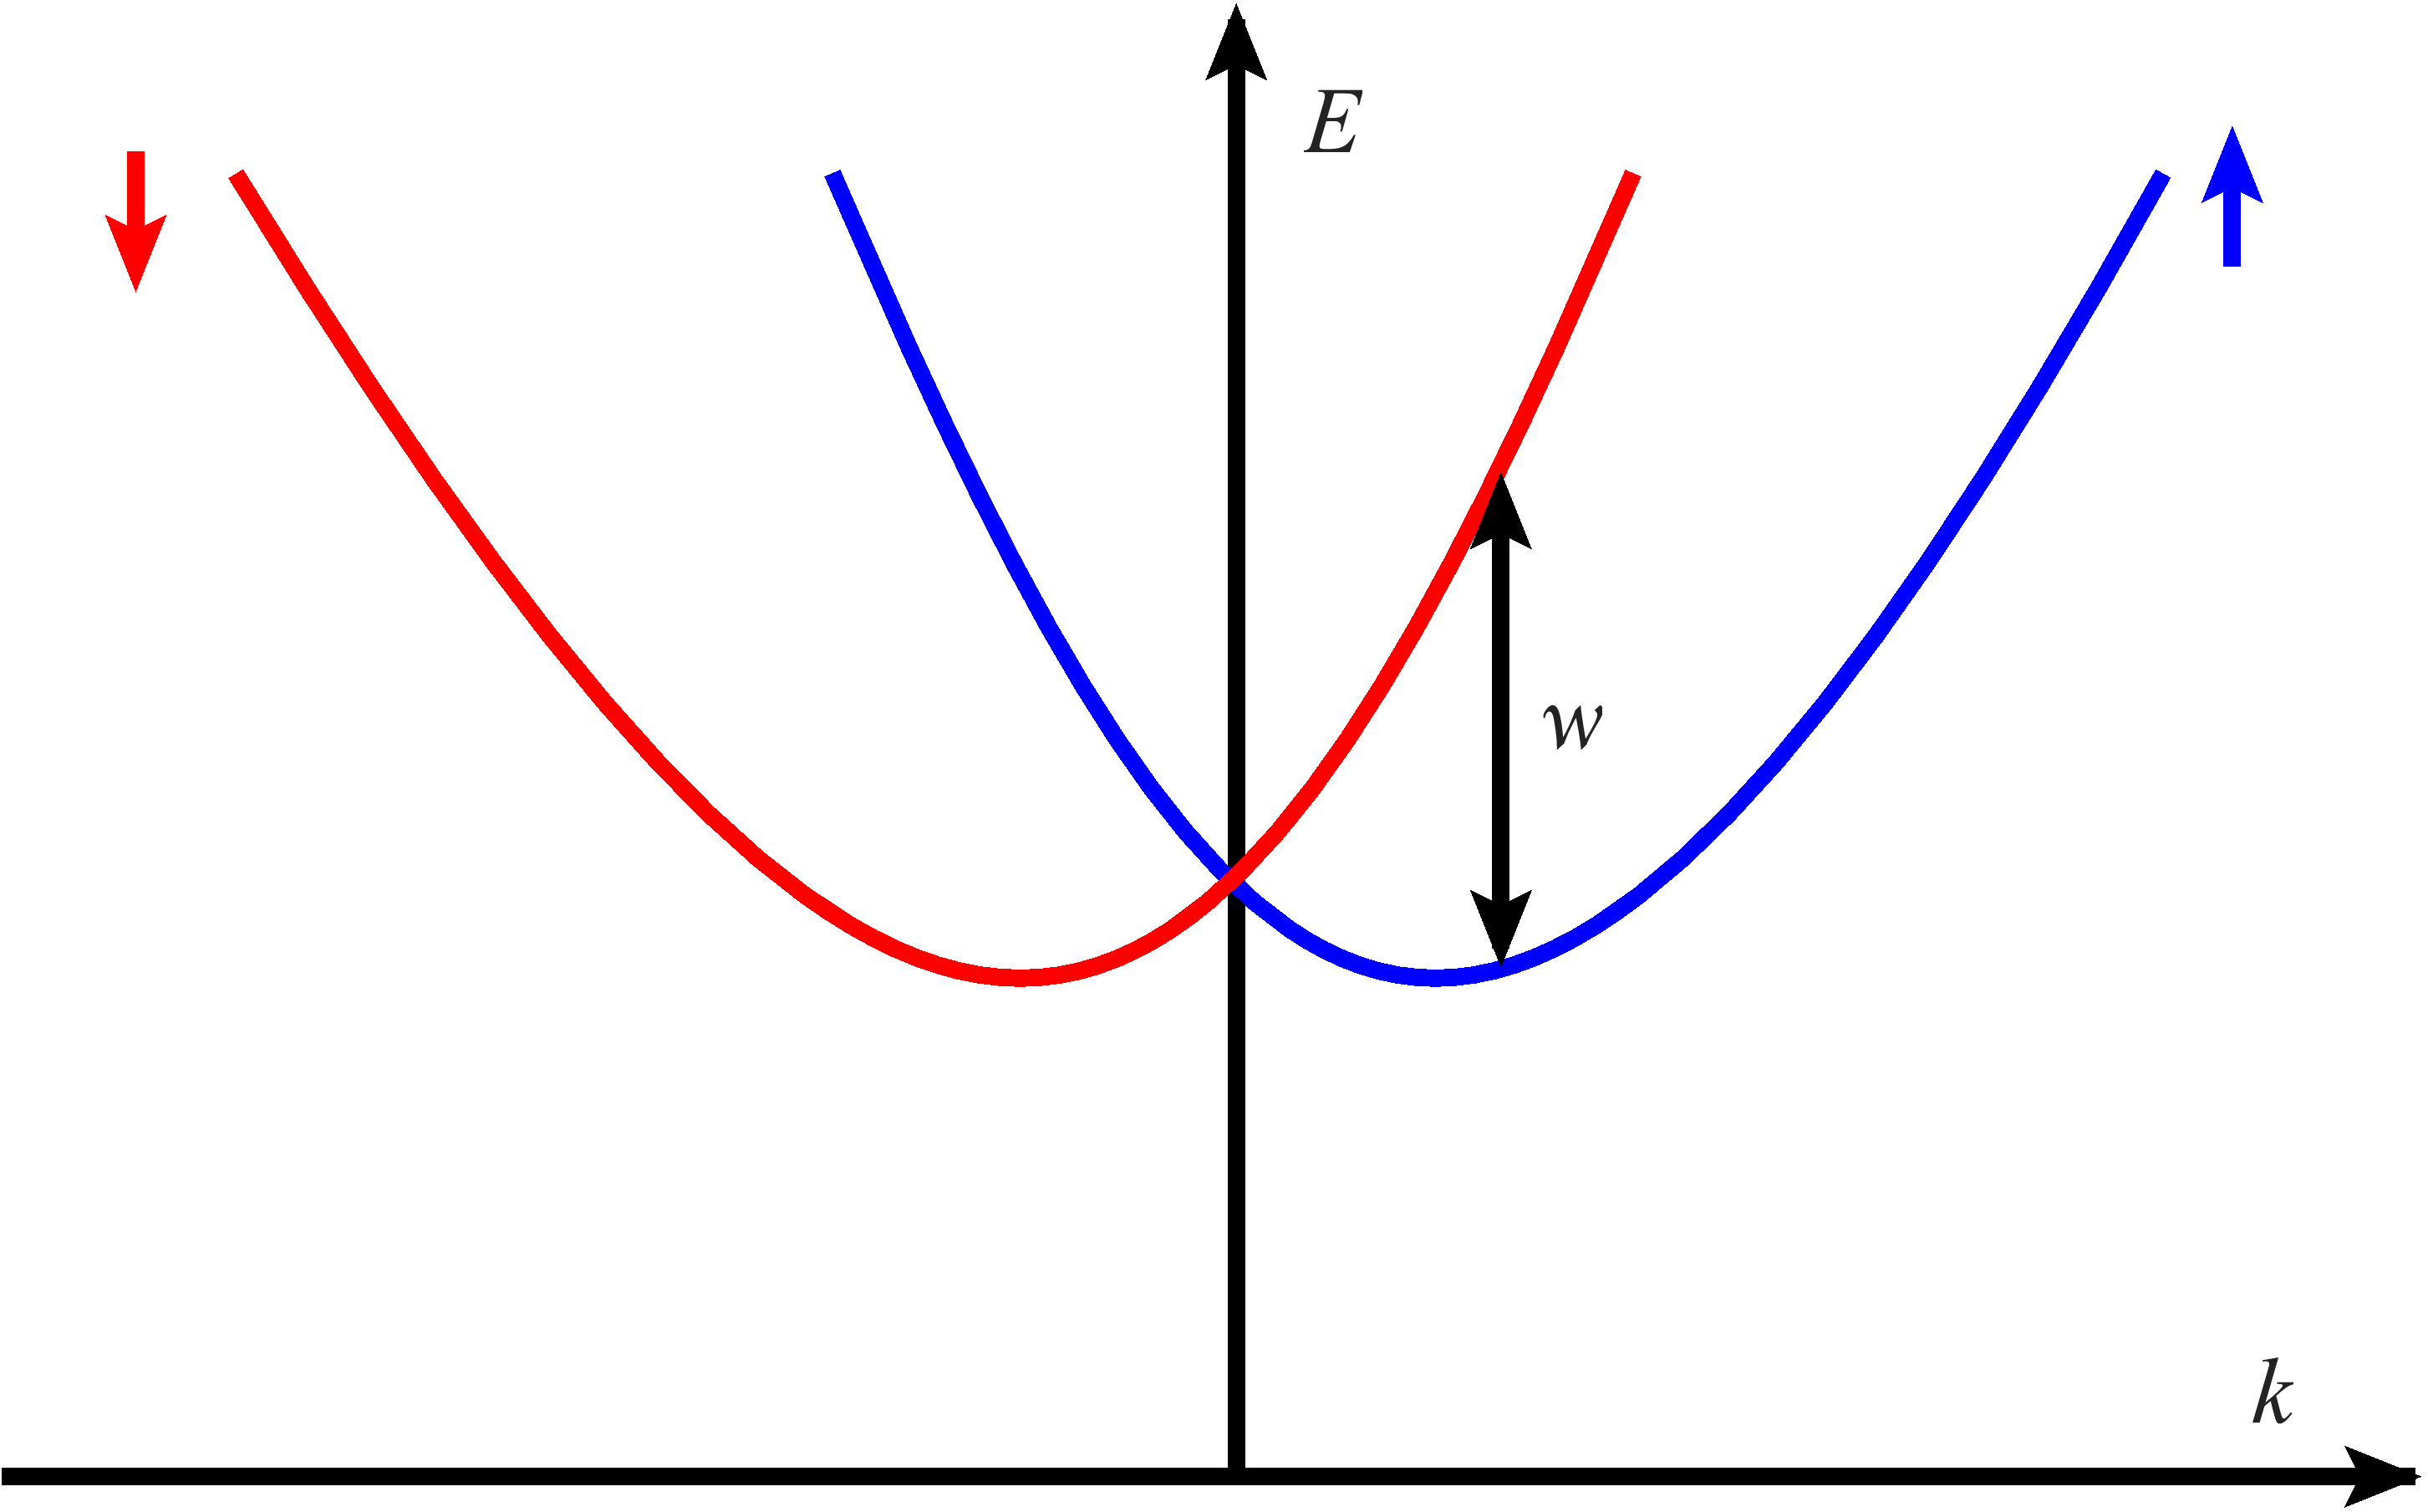
\includegraphics[scale=0.08]{DP_Ek.png} 
\caption{No inversion symmetry: model energy dispersion}
\end{figure}

This means that for a given wavevector ${\bm k}$, spin up and down are not degenerate. Thus we can think of spin-orbit coupling to be an effective ${\bm k}$-dependent magnetic field.
\begin{equation}
H_{SO}=\dfrac{1}{2} {\bm \Omega}({\bm k})\cdot{\bm \sigma}
\end{equation}
Thus in presence of any momentum scattering, the electron sees different effective fields and precesses. This random-walk like precession leads to spin relaxation.

In presence of a constant magnetic field, the phase of an electron increases linearly with time with slope set by the Larmor frequency. For substantial phase randomization, we need larger $\tau$, else the deviation of phase from the constant magnetic field line is not significant. Thus 
\begin{equation}
\tau_{DP}^{-1} \propto \tau \propto 1/T
\end{equation}
\begin{figure}
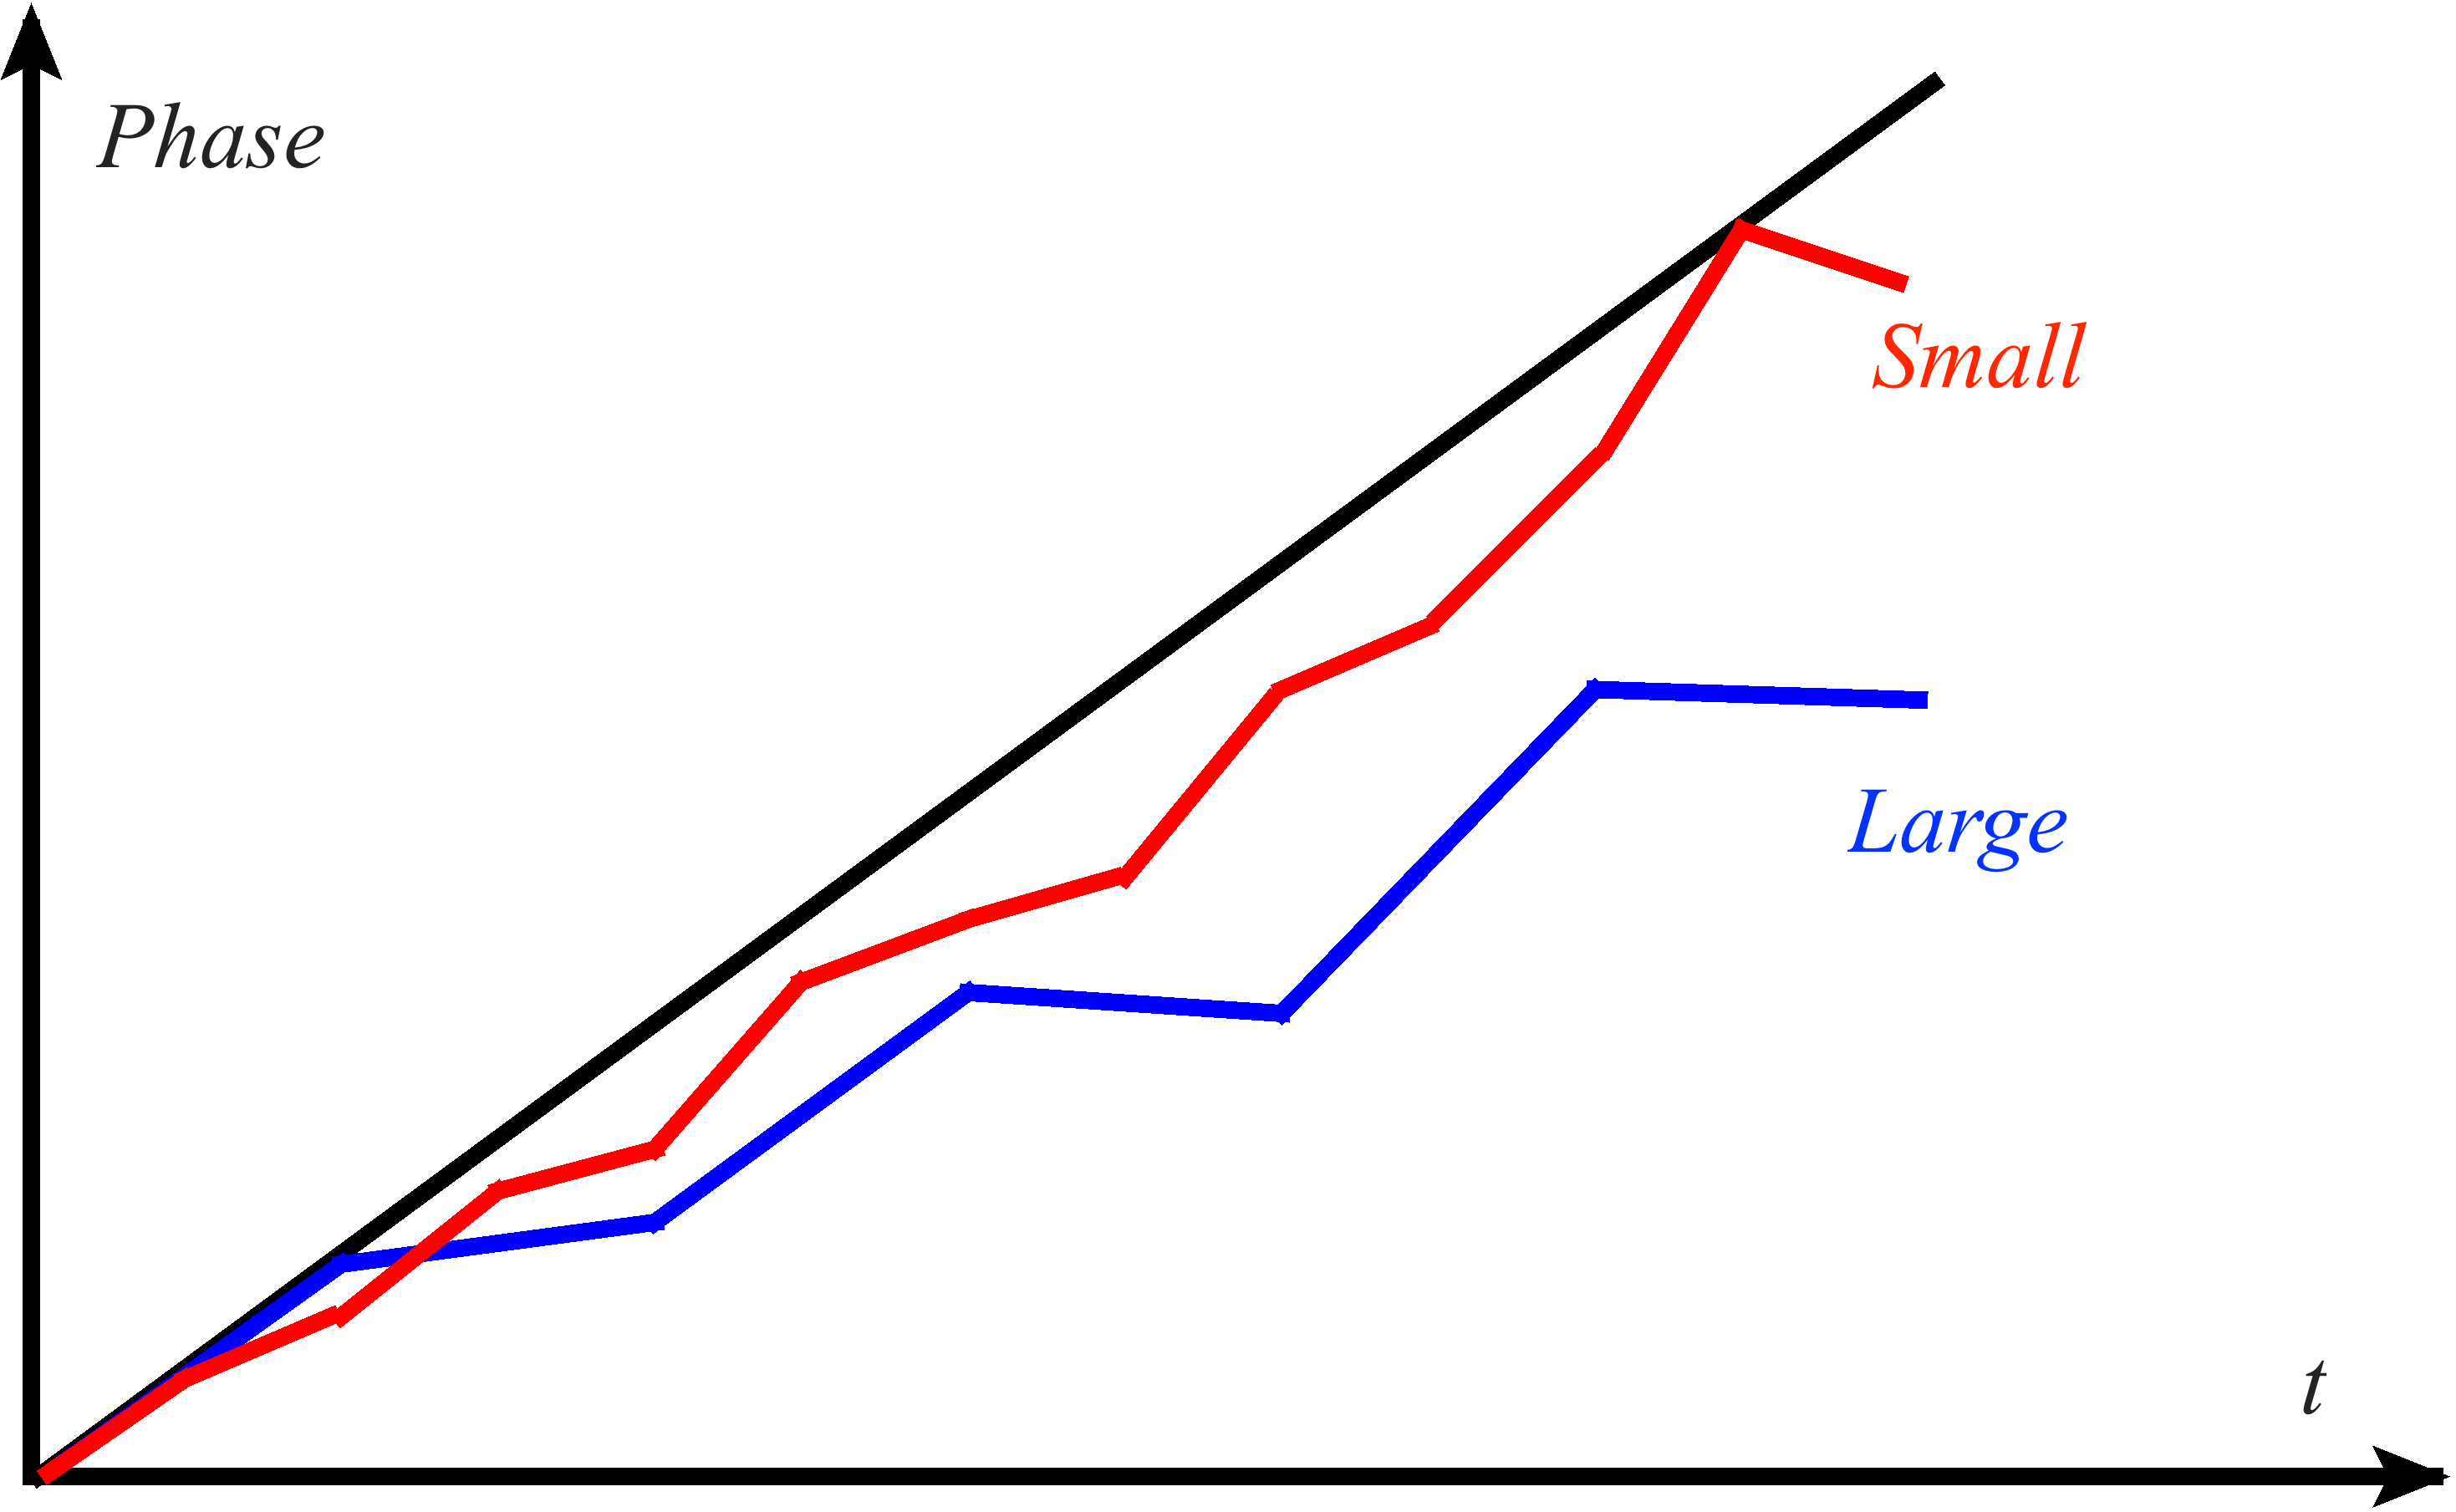
\includegraphics[scale=0.08]{DP_PhaseRelax.png} 
\caption{Dyakanov-Perel phase relaxation. Small momentum relaxation time (red) and large momentum relaxation time (blue). Clearly the large $\tau$ deviates more and leads to more spin relaxation compared to small $\tau$. This is counter intuitive and opposite to Elliot-Yafet. }
\end{figure}
\end{document}